% ============================================================
%  J4 — MATIN : Tokenisation & Word Embeddings
%  Julien Rolland — M2 Développement Fullstack
% ============================================================
\documentclass[aspectratio=169, 10pt]{beamer}
% ============================================================
%  PREAMBLE COMMUN — IA, Deep Learning & Machine Learning
%  Julien Rolland — M2 Développement Fullstack
% ============================================================

% --- Langue & encodage ---
\usepackage[utf8]{inputenc}
\usepackage[T1]{fontenc}
\usepackage{babel}
\babelprovide[import, main]{french}

% --- Thème Beamer ---
\usetheme{Madrid}
\usecolortheme{default}

% Palette de bleu académique
\definecolor{jedy_blue}{RGB}{0, 51, 102}       % bleu foncé principal
\definecolor{jedy_mid}{RGB}{0, 102, 179}        % bleu moyen accent
\definecolor{jedy_light}{RGB}{204, 221, 240}    % bleu très clair (fond boxes)
\definecolor{jedy_alert}{RGB}{180, 30, 30}      % rouge pour alertes
\definecolor{jedy_example}{RGB}{0, 120, 60}     % vert pour exemples

% Application des couleurs sur le thème Madrid
\setbeamercolor{palette primary}{bg=jedy_blue, fg=white}
\setbeamercolor{palette secondary}{bg=jedy_mid, fg=white}
\setbeamercolor{palette tertiary}{bg=jedy_blue, fg=white}
\setbeamercolor{palette quaternary}{bg=jedy_blue, fg=white}
\setbeamercolor{structure}{fg=jedy_blue}
\setbeamercolor{frametitle}{bg=jedy_blue, fg=white}
\setbeamercolor{title}{bg=jedy_blue, fg=white}
\setbeamercolor{block title}{bg=jedy_mid, fg=white}
\setbeamercolor{block body}{bg=jedy_light, fg=black}
\setbeamercolor{block title alerted}{bg=jedy_alert, fg=white}
\setbeamercolor{block body alerted}{bg=jedy_light, fg=black}
\setbeamercolor{block title example}{bg=jedy_example, fg=white}
\setbeamercolor{block body example}{bg=jedy_light, fg=black}

% --- Typographie ---
\usepackage{lmodern}
\setbeamerfont{title}{size=\Large, series=\bfseries}
\setbeamerfont{frametitle}{size=\normalsize, series=\bfseries}

% --- Navigation : suppression des icônes de navigation par défaut ---
\setbeamertemplate{navigation symbols}{}

% --- Numérotation des slides ---
\setbeamertemplate{footline}{%
  \leavevmode%
  \hbox{%
    \begin{beamercolorbox}[wd=.333\paperwidth,ht=2.25ex,dp=1ex,center]{author in head/foot}%
      \usebeamerfont{author in head/foot}\insertshortauthor
    \end{beamercolorbox}%
    \begin{beamercolorbox}[wd=.334\paperwidth,ht=2.25ex,dp=1ex,center]{title in head/foot}%
      \usebeamerfont{title in head/foot}\insertshorttitle
    \end{beamercolorbox}%
    \begin{beamercolorbox}[wd=.333\paperwidth,ht=2.25ex,dp=1ex,right]{date in head/foot}%
      \usebeamerfont{date in head/foot}
      \insertframenumber{} / \inserttotalframenumber\hspace*{2ex}
    \end{beamercolorbox}%
  }%
  \vskip0pt%
}

% --- Maths ---
\usepackage{amsmath, amssymb, amsthm}
\usepackage{bm}          % vecteurs en gras : \bm{w}

% --- Code source ---
\usepackage{listings}
\usepackage{xcolor}

\lstdefinestyle{pythonstyle}{
  language=Python,
  basicstyle=\ttfamily\footnotesize,
  keywordstyle=\color{jedy_blue}\bfseries,
  commentstyle=\color{gray}\itshape,
  stringstyle=\color{jedy_example},
  numberstyle=\tiny\color{gray},
  numbers=left,
  numbersep=5pt,
  frame=single,
  framerule=0.4pt,
  rulecolor=\color{jedy_light},
  backgroundcolor=\color{jedy_light!40},
  breaklines=true,
  showstringspaces=false,
  tabsize=4,
}
\lstset{style=pythonstyle}

% Alias pratique pour code inline
\newcommand{\code}[1]{\texttt{\small#1}}

% --- Graphiques ---
\usepackage{graphicx}
\usepackage{tikz}
\usetikzlibrary{arrows.meta, positioning, shapes.geometric, fit, calc}
\usepackage{pgfplots}
\pgfplotsset{compat=1.18}

% --- Tableaux ---
\usepackage{booktabs}
\usepackage{array}

% --- Icônes (optionnel, nécessite fontawesome5) ---
% \usepackage{fontawesome5}

% --- Macros ML/DL courantes ---
\newcommand{\R}{\mathbb{R}}
\newcommand{\E}{\mathbb{E}}
\newcommand{\Loss}{\mathcal{L}}
\newcommand{\dataset}{\mathcal{D}}
\newcommand{\X}{\mathbf{X}}
\newcommand{\y}{\mathbf{y}}
\newcommand{\w}{\mathbf{w}}
\newcommand{\W}{\mathbf{W}}
\newcommand{\grad}{\nabla}
\newcommand{\T}{^{\top}}         % transposée : \X\T
\newcommand{\lr}{\alpha}         % learning rate
\newcommand{\norm}[1]{\left\|#1\right\|}

% Encadré "Objectif pédagogique" en début de section
\newenvironment{objectif}{%
  \begin{alertblock}{Objectif}%
}{%
  \end{alertblock}%
}

% --- Infos du cours (remplacer dans chaque slides.tex) ---
\author[J. Rolland]{Julien Rolland}
\institute[Jedy]{Formation M2 Développement Fullstack}


\title[Embeddings]{Tokenisation \& Word Embeddings}
\subtitle{Jour 4 --- Matin}
\date{Jour 4}

% ============================================================
\begin{document}
% ============================================================

\begin{frame}
  \titlepage
\end{frame}

\begin{frame}{Plan du module}
  \tableofcontents
\end{frame}

% ============================================================
\section{Du texte aux nombres}
% ============================================================

\begin{frame}{Le défi du langage naturel}
  \begin{columns}[T]
    \begin{column}{0.52\textwidth}
      \begin{alertblock}{Le problème}
        \begin{itemize}
          \item Image : grille de \textbf{pixels} $=$ nombres réels $\in [0,1]$
          \item Texte : suite de \textbf{symboles discrets}
          \item Comment calculer la «~dérivée~» d'un mot ?
          \item Comment gérer la \textbf{polysémie} ?
        \end{itemize}
      \end{alertblock}
      \smallskip
      \begin{exampleblock}{Objectif du matin}
        Construire un \textbf{pont} entre le monde discret (mots)
        et le monde continu ($\mathbb{R}^d$), afin que les
        réseaux de neurones puissent traiter du texte.
      \end{exampleblock}
    \end{column}
    \begin{column}{0.44\textwidth}
      \centering
      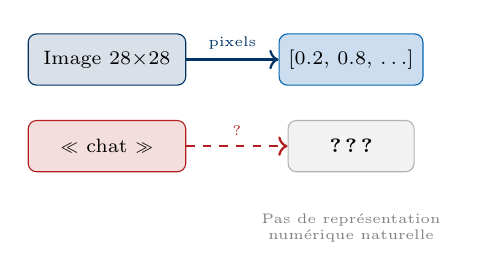
\begin{tikzpicture}[font=\scriptsize,
        box/.style={draw, rounded corners=3pt, align=center,
                    minimum width=2.0cm, minimum height=0.65cm}]
        % Image row
        \node[box, fill=jedy_blue!15, draw=jedy_blue] (img) at (0, 1.8)
          {Image $28{\times}28$};
        \node[box, fill=jedy_light, draw=jedy_mid, minimum width=1.6cm] (pix)
          at (3.1, 1.8) {$[0.2,\,0.8,\,\ldots]$};
        \draw[->, thick, jedy_blue] (img.east) -- (pix.west)
          node[midway, above, font=\tiny] {pixels};
        % Text row
        \node[box, fill=jedy_alert!15, draw=jedy_alert] (txt) at (0, 0.7)
          {«~chat~»};
        \node[box, fill=gray!10, draw=gray!60, minimum width=1.6cm] (qst)
          at (3.1, 0.7) {$\boldsymbol{?}\,\boldsymbol{?}\,\boldsymbol{?}$};
        \draw[->, thick, jedy_alert, dashed] (txt.east) -- (qst.west)
          node[midway, above, font=\tiny, color=jedy_alert] {?};
        % Caption
        \node[below=0.4cm of qst, font=\tiny, color=gray, align=center]
          {Pas de représentation\\numérique naturelle};
      \end{tikzpicture}
    \end{column}
  \end{columns}
\end{frame}

\begin{frame}{Tokenisation (1/2) --- Approches naïves}
  \begin{columns}[T]
    \begin{column}{0.48\textwidth}
      \begin{block}{Niveau caractère}
        \begin{itemize}
          \item[\textcolor{jedy_example}{$+$}] Petit vocabulaire ($\sim$256)
          \item[\textcolor{jedy_example}{$+$}] Aucun mot inconnu (OOV)
          \item[\textcolor{jedy_alert}{$-$}] Perte de la sémantique locale
          \item[\textcolor{jedy_alert}{$-$}] Séquences très longues
        \end{itemize}
        \smallskip
        \code{chat} $\;\to\;$ \texttt{\small[c, h, a, t]}
      \end{block}
    \end{column}
    \begin{column}{0.48\textwidth}
      \begin{block}{Niveau mot (\textit{word-level})}
        \begin{itemize}
          \item[\textcolor{jedy_example}{$+$}] Sens clair, séquences courtes
          \item[\textcolor{jedy_alert}{$-$}] Vocabulaire immense ($V > 100\,000$)
          \item[\textcolor{jedy_alert}{$-$}] Mots hors dictionnaire (OOV)
          \item[\textcolor{jedy_alert}{$-$}] Flexions = tokens distincts
        \end{itemize}
        \smallskip
        «~mangeras~» $\ne$ «~mangeons~»
      \end{block}
    \end{column}
  \end{columns}
  \bigskip
  \begin{alertblock}{Le dilemme}
    Caractère : trop fin \quad---\quad Mot : trop grossier
    \quad$\Rightarrow$\quad Y a-t-il un juste milieu ?
  \end{alertblock}
\end{frame}

\begin{frame}{Tokenisation (2/2) --- Subword : Byte Pair Encoding}
  \begin{columns}[T]
    \begin{column}{0.50\textwidth}
      \begin{block}{Principe du BPE}
        \begin{enumerate}
          \item Initialiser : chaque caractère est un token
          \item Compter les \textbf{paires} adjacentes les plus fréquentes
          \item Fusionner la paire la plus fréquente $\to$ nouveau token
          \item Répéter jusqu'à la taille de vocabulaire cible
        \end{enumerate}
      \end{block}
      \smallskip
      \begin{block}{Résultat}
        Mots \textbf{fréquents} conservés entiers.\\
        Mots \textbf{rares} découpés en sous-mots significatifs.
      \end{block}
    \end{column}
    \begin{column}{0.46\textwidth}
      \begin{exampleblock}{Exemple}
        \centering
        \vspace{4pt}
        \small «~inexplicablement~»\\[6pt]
        $\downarrow$\\[4pt]
        \texttt{\small[in \,|\, explicable \,|\, ment]}
        \vspace{4pt}
      \end{exampleblock}
      \smallskip
      \begin{alertblock}{Vocabulaires modernes}
        \begin{itemize}
          \item GPT-2 : 50\,257 tokens (BPE)
          \item BERT : 30\,522 tokens (WordPiece)
          \item Couvrent \textbf{n'importe quel} texte
        \end{itemize}
      \end{alertblock}
    \end{column}
  \end{columns}
\end{frame}

% ============================================================
\section{One-Hot vs embeddings denses}
% ============================================================

\begin{frame}{Vectorisation naïve : \textit{One-Hot Encoding}}
  \begin{columns}[T]
    \begin{column}{0.36\textwidth}
      \centering
      \vspace{4pt}
      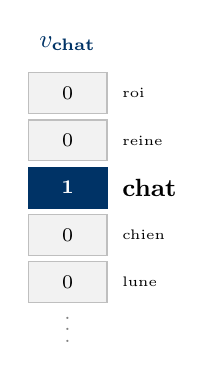
\begin{tikzpicture}[
        gz/.style={draw=gray!50, fill=gray!10,
                   minimum width=1.0cm, minimum height=0.52cm},
        hl/.style={draw=jedy_blue, fill=jedy_blue, text=white,
                   minimum width=1.0cm, minimum height=0.52cm}]
        \node[gz] (r0) at (0, 0.00) {\scriptsize 0};
          \node[anchor=west, font=\tiny] at (0.57, 0.00) {roi};
        \node[gz] (r1) at (0,-0.60) {\scriptsize 0};
          \node[anchor=west, font=\tiny] at (0.57,-0.60) {reine};
        \node[hl] (r2) at (0,-1.20) {\scriptsize\textbf{1}};
          \node[anchor=west, font=\small\bfseries] at (0.57,-1.20) {chat};
        \node[gz] (r3) at (0,-1.80) {\scriptsize 0};
          \node[anchor=west, font=\tiny] at (0.57,-1.80) {chien};
        \node[gz] (r4) at (0,-2.40) {\scriptsize 0};
          \node[anchor=west, font=\tiny] at (0.57,-2.40) {lune};
        \node[font=\scriptsize, color=gray] at (0,-2.90) {$\vdots$};
        \node[above=0.15cm of r0, font=\small\bfseries, color=jedy_blue]
          {$v_{\text{chat}}$};
      \end{tikzpicture}
    \end{column}
    \begin{column}{0.60\textwidth}
      \begin{alertblock}{Les 3 fléaux du One-Hot}
        \begin{enumerate}
          \item \textbf{Creusité} : $V = 50\,000$ valeurs, un seul \texttt{1}
          \item \textbf{Orthogonalité} :
                $v_{\text{chat}} \cdot v_{\text{chien}} = 0$ ---
                aucune notion de proximité sémantique
          \item \textbf{Dimensionnalité} : taille vecteur $=$ taille vocabulaire
        \end{enumerate}
      \end{alertblock}
      \smallskip
      \begin{exampleblock}{La solution : embedding dense}
        Représenter chaque token par un vecteur \textbf{dense}
        de petite dimension $d \ll V$\,:
        \[
          d \in \{64,\; 128,\; 256,\; 768,\; \ldots\}
        \]
      \end{exampleblock}
    \end{column}
  \end{columns}
\end{frame}

\begin{frame}{L'espace sémantique}
  \begin{columns}[T]
    \begin{column}{0.52\textwidth}
      \centering
      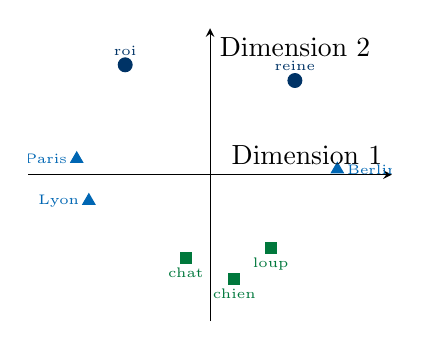
\begin{tikzpicture}
        \begin{axis}[
          width=6.2cm, height=5.3cm,
          xlabel={Dimension 1}, ylabel={Dimension 2},
          xlabel style={font=\tiny}, ylabel style={font=\tiny},
          tick style={font=\tiny},
          xmin=-3, xmax=3, ymin=-2.8, ymax=2.8,
          grid=both, grid style={gray!20},
          axis lines=center,
          xtick=\empty, ytick=\empty,
        ]
          % Royauté
          \addplot[only marks, mark=*, mark size=2.5pt, color=jedy_blue]
            coordinates {(-1.4,2.1)(1.4,1.8)};
          \node[font=\tiny, color=jedy_blue, anchor=south]
            at (axis cs:-1.4,2.1) {roi};
          \node[font=\tiny, color=jedy_blue, anchor=south]
            at (axis cs:1.4,1.8) {reine};
          % Animaux
          \addplot[only marks, mark=square*, mark size=2pt, color=jedy_example]
            coordinates {(-0.4,-1.6)(0.4,-2.0)(1.0,-1.4)};
          \node[font=\tiny, color=jedy_example, anchor=north]
            at (axis cs:-0.4,-1.6) {chat};
          \node[font=\tiny, color=jedy_example, anchor=north]
            at (axis cs:0.4,-2.0) {chien};
          \node[font=\tiny, color=jedy_example, anchor=north]
            at (axis cs:1.0,-1.4) {loup};
          % Villes
          \addplot[only marks, mark=triangle*, mark size=2.5pt, color=jedy_mid]
            coordinates {(-2.2,0.3)(-2.0,-0.5)(2.1,0.1)};
          \node[font=\tiny, color=jedy_mid, anchor=east]
            at (axis cs:-2.2,0.3) {Paris};
          \node[font=\tiny, color=jedy_mid, anchor=east]
            at (axis cs:-2.0,-0.5) {Lyon};
          \node[font=\tiny, color=jedy_mid, anchor=west]
            at (axis cs:2.1,0.1) {Berlin};
        \end{axis}
      \end{tikzpicture}
    \end{column}
    \begin{column}{0.44\textwidth}
      \begin{block}{Embedding dense $\in \R^d$}
        Chaque token est représenté par un vecteur réel\,:
        \[
          \text{chat} \;\longmapsto\;
          \begin{bmatrix} 0.31 \\ {-0.87} \\ \vdots \end{bmatrix}
          \in \R^{768}
        \]
      \end{block}
      \vspace{2pt}
      \begin{exampleblock}{Intuition géométrique}
        Les \textbf{dimensions} encodent des traits latents :\\
        genre, animité, géographie, abstraction\ldots\\[3pt]
        Le sens devient une \textbf{position} dans l'espace :
        mots proches sémantiquement $=$ proches géométriquement.
      \end{exampleblock}
    \end{column}
  \end{columns}
\end{frame}

% ============================================================
\section{Word2Vec \& propriétés}
% ============================================================

\begin{frame}{Apprendre l'espace : Word2Vec}
  \begin{columns}[T]
    \begin{column}{0.52\textwidth}
      \begin{block}{L'hypothèse distributionnelle}
        «~On connaît un mot par ses voisins.~»\\[6pt]
        \textit{«~le \underline{chat} dort sur le tapis~»}\\[2pt]
        $\Rightarrow$ «~chat~» cooccure avec : dormir, tapis, \ldots
      \end{block}
      \smallskip
      \begin{block}{Méthode Skip-gram}
        \begin{enumerate}
          \item Fenêtre glissante (taille $k$) sur le corpus
          \item Réseau : prédire les mots \textbf{contexte} à partir
                du mot \textbf{cible}
          \item Matrice de poids $\W_{e} \in \R^{V \times d}$
                $=$ dictionnaire d'embeddings
          \item[\,$\star$] On \textbf{jette la prédiction} et ne
                conserve que $\W_{e}$
        \end{enumerate}
      \end{block}
    \end{column}
    \begin{column}{0.44\textwidth}
      \centering
      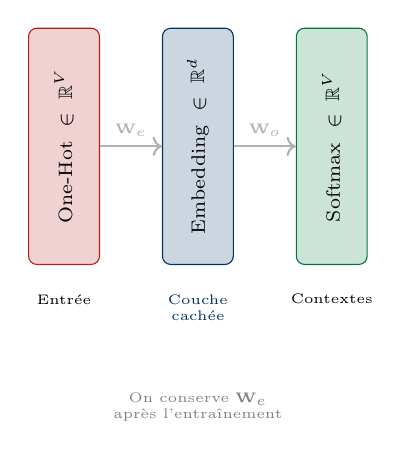
\begin{tikzpicture}[font=\scriptsize,
        nd/.style={draw, rounded corners=3pt, minimum width=0.9cm,
                   minimum height=3.0cm, align=center},
        arr/.style={->, thick, gray!60}]
        % Couches
        \node[nd, fill=jedy_alert!20, draw=jedy_alert] (inp) at (0,0)
          {\rotatebox{90}{One-Hot $\;\in\;\R^V$}};
        \node[nd, fill=jedy_blue!20, draw=jedy_blue] (emb) at (1.7,0)
          {\rotatebox{90}{Embedding $\;\in\;\R^d$}};
        \node[nd, fill=jedy_example!20, draw=jedy_example] (out) at (3.4,0)
          {\rotatebox{90}{Softmax $\;\in\;\R^V$}};
        % Flèches
        \draw[arr] (inp.east) -- (emb.west)
          node[midway, above, font=\tiny] {$\W_e$};
        \draw[arr] (emb.east) -- (out.west)
          node[midway, above, font=\tiny] {$\W_o$};
        % Labels
        \node[below=0.25cm of inp, font=\tiny, align=center] {Entrée};
        \node[below=0.25cm of emb, font=\tiny, align=center, color=jedy_blue]
          {Couche\\cachée};
        \node[below=0.25cm of out, font=\tiny, align=center] {Contextes};
        % Note
        \node[below=1.5cm of emb, font=\tiny, color=gray, align=center,
              text width=2.5cm]
          {On conserve $\W_e$ après l'entraînement};
      \end{tikzpicture}
    \end{column}
  \end{columns}
\end{frame}

\begin{frame}{Algèbre de mots \& similarité cosinus}
  \begin{columns}[T]
    \begin{column}{0.52\textwidth}
      \begin{exampleblock}{Propriété : analogies vectorielles}
        Les relations sémantiques $=$ translations dans $\R^d$ :
        \[
          \vec{\text{roi}} - \vec{\text{homme}} + \vec{\text{femme}}
          \;\approx\; \vec{\text{reine}}
        \]
        \[
          \vec{\text{Paris}} - \vec{\text{France}} + \vec{\text{Allemagne}}
          \;\approx\; \vec{\text{Berlin}}
        \]
      \end{exampleblock}
      \smallskip
      \begin{block}{Mesure de proximité : similarité cosinus}
        \[
          \cos(\theta) = \frac{A \cdot B}{\norm{A}\,\norm{B}}
          \;\in\; [-1,\;1]
        \]
        \vspace{-6pt}
        \begin{center}
          \footnotesize
          $1$ : synonymes \quad $0$ : sans rapport \quad $-1$ : antonymes
        \end{center}
      \end{block}
    \end{column}
    \begin{column}{0.44\textwidth}
      \centering
      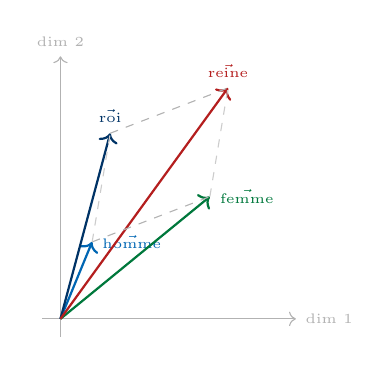
\begin{tikzpicture}[font=\tiny, scale=1.15]
        \draw[->, gray!60] (-0.2,0) -- (2.6,0) node[right] {dim 1};
        \draw[->, gray!60] (0,-0.2) -- (0,2.9) node[above] {dim 2};
        % Vecteurs depuis l'origine
        \draw[->, thick, jedy_mid]     (0,0) -- (0.35,0.85)
          node[right] {$\vec{\text{homme}}$};
        \draw[->, thick, jedy_blue]    (0,0) -- (0.55,2.05)
          node[above] {$\vec{\text{roi}}$};
        \draw[->, thick, jedy_example] (0,0) -- (1.65,1.35)
          node[right] {$\vec{\text{femme}}$};
        \draw[->, thick, jedy_alert]   (0,0) -- (1.85,2.55)
          node[above] {$\vec{\text{reine}}$};
        % Parallélogramme (tirets)
        \draw[dashed, gray!60] (0.55,2.05) -- (1.85,2.55);
        \draw[dashed, gray!60] (0.35,0.85) -- (1.65,1.35);
        \draw[dashed, gray!40] (0.35,0.85) -- (0.55,2.05);
        \draw[dashed, gray!40] (1.65,1.35) -- (1.85,2.55);
      \end{tikzpicture}
    \end{column}
  \end{columns}
\end{frame}

% ============================================================
\section{Visualisation \& limites}
% ============================================================

\begin{frame}{Visualisation : réduction de dimension (t-SNE)}
  \begin{columns}[T]
    \begin{column}{0.54\textwidth}
      \centering
      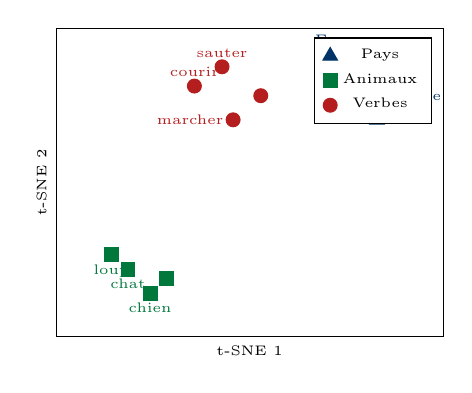
\begin{tikzpicture}
        \begin{axis}[
          width=6.5cm, height=5.5cm,
          xlabel={t-SNE 1}, ylabel={t-SNE 2},
          xlabel style={font=\tiny}, ylabel style={font=\tiny},
          tick style={font=\tiny},
          xmin=-3.5, xmax=3.5, ymin=-3.2, ymax=3.2,
          grid=both, grid style={gray!15},
          xtick=\empty, ytick=\empty,
          legend pos=north east,
          legend style={font=\tiny, cells={align=left}},
        ]
          % Pays
          \addplot[only marks, mark=triangle*, mark size=3pt, color=jedy_blue]
            coordinates {(2.1,2.2)(2.5,1.8)(1.8,2.6)(2.3,1.3)};
          \addlegendentry{Pays}
          % Animaux
          \addplot[only marks, mark=square*, mark size=2.5pt, color=jedy_example]
            coordinates {(-2.2,-1.8)(-1.8,-2.3)(-2.5,-1.5)(-1.5,-2.0)};
          \addlegendentry{Animaux}
          % Verbes
          \addplot[only marks, mark=*, mark size=2.5pt, color=jedy_alert]
            coordinates {(-1.0,2.0)(-0.5,2.4)(0.2,1.8)(-0.3,1.3)};
          \addlegendentry{Verbes}
          % Labels
          \node[color=jedy_blue,    font=\tiny, anchor=south]
            at (axis cs:2.1,2.2)   {France};
          \node[color=jedy_blue,    font=\tiny, anchor=west]
            at (axis cs:2.5,1.8)   {Italie};
          \node[color=jedy_blue,    font=\tiny, anchor=south]
            at (axis cs:1.8,2.6)   {Espagne};
          \node[color=jedy_example, font=\tiny, anchor=north]
            at (axis cs:-2.2,-1.8) {chat};
          \node[color=jedy_example, font=\tiny, anchor=north]
            at (axis cs:-1.8,-2.3) {chien};
          \node[color=jedy_example, font=\tiny, anchor=north]
            at (axis cs:-2.5,-1.5) {loup};
          \node[color=jedy_alert,   font=\tiny, anchor=south]
            at (axis cs:-1.0,2.0)  {courir};
          \node[color=jedy_alert,   font=\tiny, anchor=south]
            at (axis cs:-0.5,2.4)  {sauter};
          \node[color=jedy_alert,   font=\tiny, anchor=east]
            at (axis cs:-0.3,1.3)  {marcher};
        \end{axis}
      \end{tikzpicture}
    \end{column}
    \begin{column}{0.42\textwidth}
      \begin{block}{Le problème}
        Embeddings $\in \R^{768}$ :\\
        impossible à visualiser directement.
      \end{block}
      \smallskip
      \begin{exampleblock}{t-SNE / UMAP}
        \begin{itemize}
          \item Projection en 2D
          \item \textbf{Préserve la structure locale}
                des voisinages
          \item Les clusters révèlent les
                \textbf{classes sémantiques}
        \end{itemize}
      \end{exampleblock}
      \vspace{2pt}
      \begin{alertblock}{Attention}
        t-SNE préserve la \textbf{proximité locale},
        pas les distances globales.
      \end{alertblock}
    \end{column}
  \end{columns}
\end{frame}

\begin{frame}{Limites des embeddings statiques}
  \begin{columns}[T]
    \begin{column}{0.52\textwidth}
      \begin{alertblock}{Le problème : la polysémie}
        \begin{itemize}
          \item «~Je dépose de l'argent à la \textbf{banque}.~»
          \item «~Je pêche au bord de la \textbf{banque}.~»
        \end{itemize}
        \vspace{4pt}
        Dans Word2Vec / GloVe, «~banque~» possède
        \textbf{un seul vecteur}, mélangeant les deux sens.
      \end{alertblock}
      \smallskip
      \begin{alertblock}{Autres limites}
        \begin{itemize}
          \item Ignorent l'ordre des mots
          \item Embeddings \textbf{figés} après entraînement
          \item Biais hérités des données d'entraînement
        \end{itemize}
      \end{alertblock}
    \end{column}
    \begin{column}{0.44\textwidth}
      \begin{block}{La solution : embeddings \textbf{contextuels}}
        Le vecteur d'un mot doit dépendre de son \textbf{contexte}.
        \vspace{4pt}
        \begin{center}
          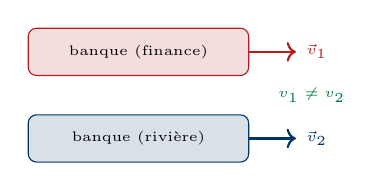
\begin{tikzpicture}[font=\tiny,
            box/.style={draw, rounded corners=3pt, align=center,
                        minimum width=2.8cm, minimum height=0.6cm}]
            \node[box, fill=jedy_alert!15, draw=jedy_alert] (b1) at (0,0)
              {banque (finance)};
            \node[box, fill=jedy_blue!15, draw=jedy_blue] (b2) at (0,-1.1)
              {banque (rivi\`ere)};
            \draw[->, jedy_alert, thick] (b1.east) -- (2.0, 0.0)
              node[right] {$\vec{v}_1$};
            \draw[->, jedy_blue, thick]  (b2.east) -- (2.0,-1.1)
              node[right] {$\vec{v}_2$};
            \node[font=\tiny\bfseries, color=jedy_example] at (2.2,-0.55)
              {$v_1 \neq v_2$};
          \end{tikzpicture}
        \end{center}
      \end{block}
      \vspace{2pt}
      \begin{exampleblock}{J4-PM $\;\to\;$ mécanisme d'attention}
        L'attention permet de construire des embeddings
        \textbf{dynamiques} selon le contexte.
      \end{exampleblock}
    \end{column}
  \end{columns}
\end{frame}

\end{document}
